% MIRU2023 LaTeXクラスファイルの使い方 Ver.1
\documentclass[MIRU,submit,uplatex]{miru2023j}
\usepackage[dvipdfmx]{graphicx}
\usepackage{latexsym}
\usepackage[fleqn]{amsmath}
\usepackage[psamsfonts]{amssymb}

\begin{document}

\title{順伝播型ニューラルネットワーク によるブラシスタイル変換}

\affiliate{Tokyo}{早稲田大学}
% \affiliate{Osaka}{第二大学(現在,第三コーポレーション勤務)}

 \author{木幡 咲希}{Saki KOHATA}{Tokyo}[cat-73@akane.waseda.jp]
 \author{シモセラ エドガー}{Edgar SIMO-SERRA}{Tokyo}[ess@waseda.jp]
%  \author{理解 次郎}{Jiro RIKAI}{Osaka}[jiro@rikai.co.jp]
%  \author{John Smith}{John Smith}{Osaka,Tokyo}[john@rikai.co.jp]

\maketitle

\section*{概要}
AI技術の発達により, 絵を描く技術の有無にかかわらず, 多くの人が完成度の高い絵を生成
できるようになった. しかし, AI技術を用いた絵の生成に取り組む研究のほとんどは画像
をアーティスティックなスタイルに変更したり, テキストをもとに画像を生成したりなど,
既にクリエイターとして働いている人が使えるツールであるとは言い難い. 
本研究では, 人間が描いた絵のブラシスタイルを学習し, 新たな入力画像をその学習した
ブラシスタイルを用いて再描画した画像を生成するモデルを提案する. 

\section{序論}
人間は, 絵画を通じて自分の感情や思考を表現することに価値を見出してきた.
優れた作品を生み出すためには, 構図やスケッチ技術, 色彩や照明効果などを学ぶ必要が
あり, その習得には長い時間がかかるものであった. しかし, AI技術の進歩により, 
絵を描く技術のない人にも完成度の高い絵画を生成することが可能となった.
例えば, Midjourney\cite{Midjourney}は, 描いてほしい絵のイメージを単語や文章, キーワード
で入力するだけで素晴らしい絵画を生成することができるソフトウェアである. 
Midjourneyは, 使い方が簡単であることや生成された絵画が高品質であることから
人気であり, クリエイターにも高く評価されている.
しかし, このようなツールは, すでに自分のスタイルを確立したクリエイターにとって
役に立つツールであるとは言い難い. 
クリエイターにとっては, デジタル・アナログを問わず, 自分の手で作品を作ることが
重要であり, Midjourneyのように絵の生成課程の全てがAI技術に頼ったツールでは, 
描かれたオブジェクトの形状や色合いなどに不満が残ると考えられるからである.
私たちは, クリエイターが作業の途中に使えるような, 
クリエイターの支援につながる研究を行いたいと考えた.
そこで, クリエイターが描いた絵のブラシスタイルを学習し, そのブラシスタイルを
新たな画像に適応するモデルを開発することを目標とした. 

本研究で提案したいモデルは, コンテンツ参照画像とスタイル参照画像の
2つの画像を入力とし, コンテンツ参照画像に描かれたものをスタイル参照画像の
ブラシスタイルで再描画した画像を生成するモデルである. 
図\ref{fig:haru}に, 2つの入力画像と出力画像の例を示す.
図\ref{fig:haru}に示すコンテンツ参照画像のような画像を簡単なブラシを用いて手動で
作成し, それをモデルに入力してクリエイターのブラシスタイルで再描画させることで,
クリエイターが絵の制作プロセスを大幅に効率化できることが期待される.
コンテンツ参照画像はクリエイターが作成するものであるため, オブジェクトの形や色は
クリエイターがコントロールすることができ, 生成画像に対する不満は多少の修正によって
解消できると考えられる. 
\begin{figure}
    \centering
    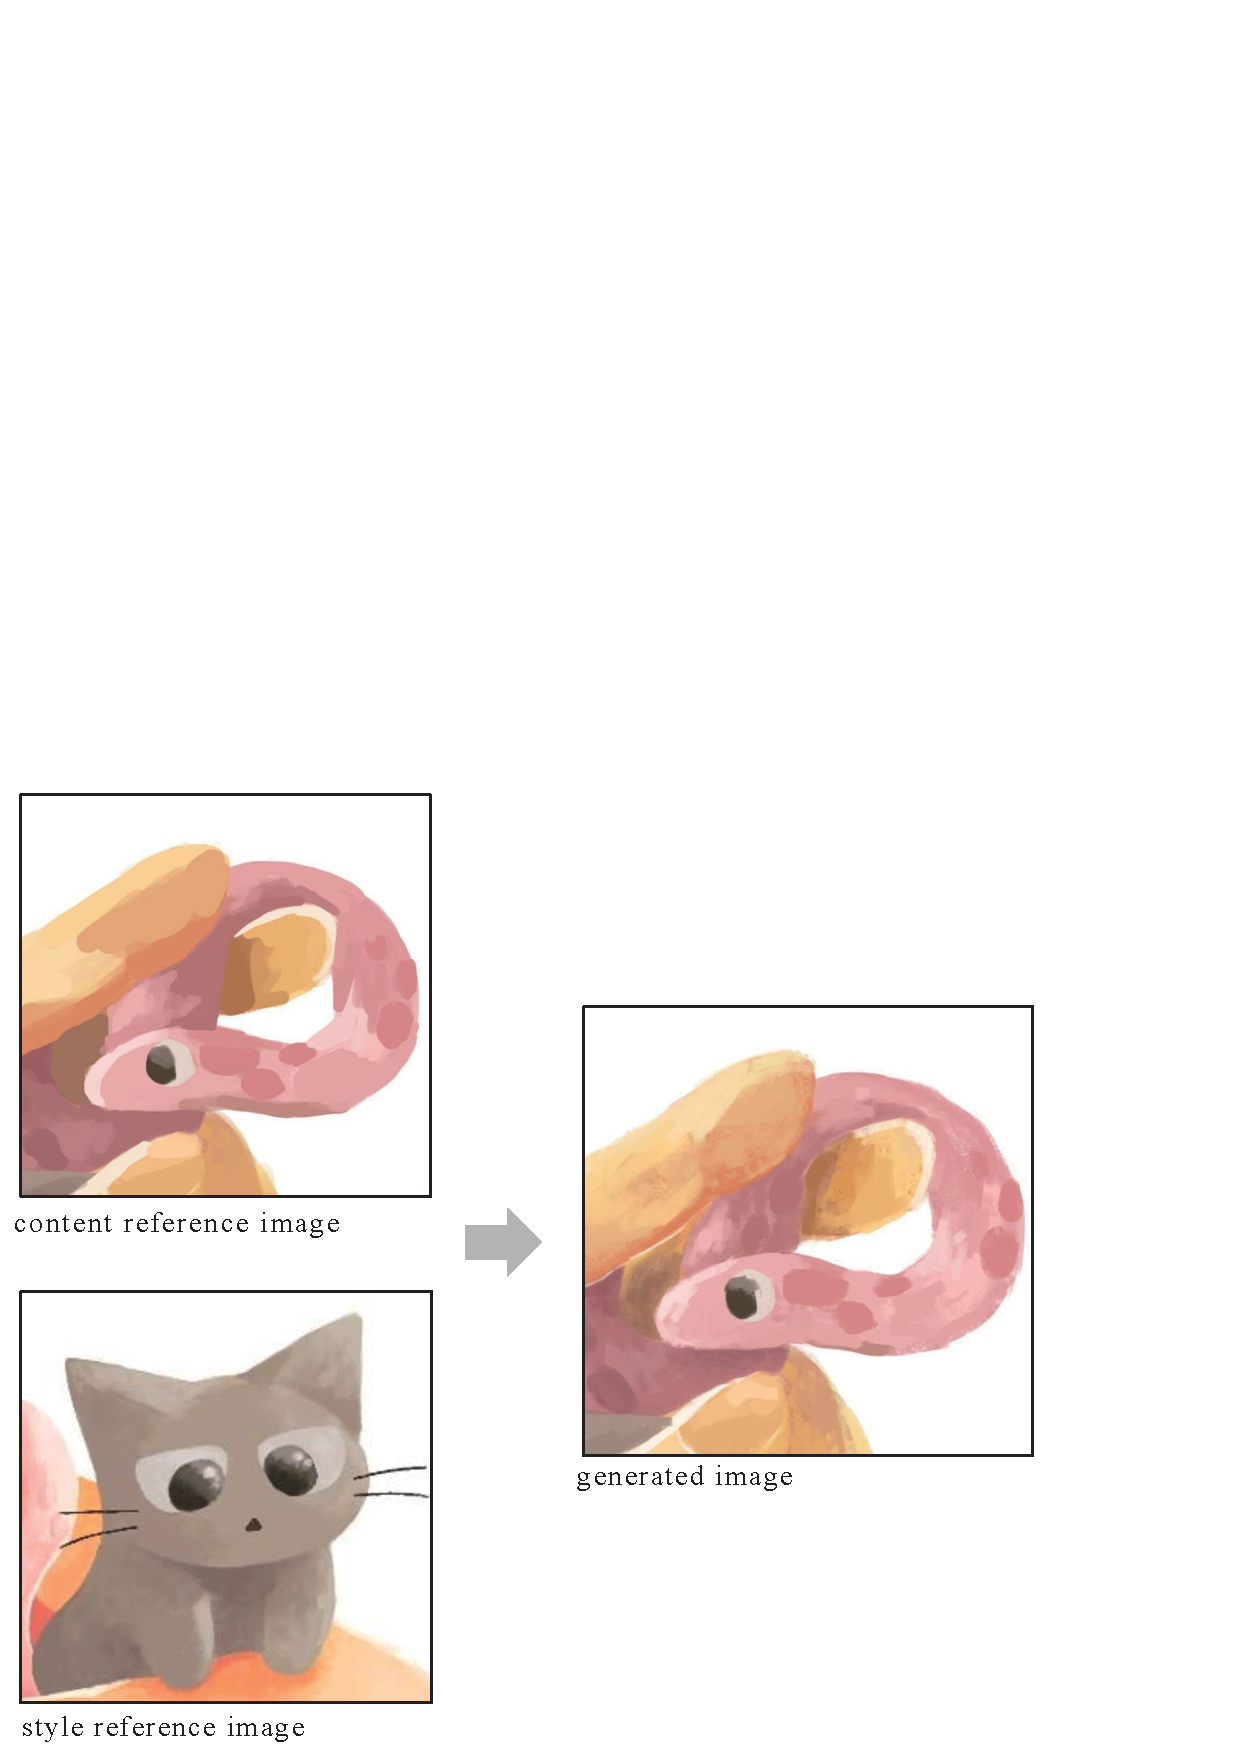
\includegraphics[width=1.0\linewidth]{resource/haru.pdf}
    \caption{作成したいモデルの入力画像と出力画像の例.}
    \label{fig:haru}
\end{figure}

\begin{figure*}[t]
    \centering
    \includegraphics[width=1.0\linewidth]{resource/future_model.pdf}
    \caption{目標のモデルの構造.}
    \label{fig:final_model}
\end{figure*}

\section{関連研究}
画像のスタイル変換という分野では, ある画像から別の画像へのスタイルの転写に関する
研究\cite{IST}が存在する. 提案されたモデルは風景写真をアーティスティックなスタイルに
変換することを可能とするが, スタイル参照画像全体の雰囲気と色をコンテンツ参照画像
にうつすものとなっている. そのため, コンテンツ参照画像には存在しない, 
スタイル参照画像に描かれた特徴的なオブジェクトが, モデルからの出力画像に出現する.
本研究では, コンテンツ参照に描かれた内容や色は変更せず, ブラシのスタイルのみを
うつすことを目的としている. 
Huangら\cite{Huang_2019_ICCV} と Liuら\cite{liu2021paint}は, 
入力画像に描かれた内容を描画するストロークを生成するモデルを提案した. 
これらはいずれも指定されたブラシによるストロークを生成するものであり, 
ブラシスタイルの模倣については取り扱っていない. 
Liuらが提案した, Transformerをベースとしたストローク生成パイプラインを本研究における
提案モデルのストローク予測モデルに採用した. 

\section{提案手法}
提案モデルでは, Liuらが提案したPaint transformer\cite{liu2021paint}という, 
Transformerベースのフレームワークをストローク予測パイプラインとして利用した.
本研究の最終目的は, コンテンツ参照画像に描かれた内容を
スタイル参照画像のブラシスタイルで再描画することであるため, ストロークパラメータと
ブラシパラメータの最適化を交互に行うモデルを作成することが最終的に目指すところ
である.
ここで, ストロークパラメータはストロークの色や大きさのような, ストロークごとに
異なるパラメータのことを指し, ブラシパラメータはベースとなるブラシ画像などの, 
すべてのストロークに共通するパラメータを指す. 
しかし, 今の段階では二重最適化の実装まで行えていない. 
以下では, まず目標のモデルの構造を説明し, 次に本論文での提案モデルの説明を行う.

\subsection{目標のモデルの構造}
ストローク予測パイプラインとして用いたPaint transformerは, Transformerベースの
フレームワークである. 
このフレームワークは, 順伝播型の変換器を用いて複数のストロークの
ストロークパラメータを予測することで, ストローク列を生成する.
Paint transformerは, ストローク予測器とストロークレンダラーという2つのモジュール
から構成されている. ストロークは位置と回転角を表す5つの形状パラメータと, RGBの
それぞれに対応する3つの色パラメータによって表現されており, 
それらをもとにベースとなるブラシ画像を変換してレンダリングされる.
したがって, Paint transformerによってレンダリングされるストロークは, 
ベースとなるブラシ画像を拡大・縮小・回転した, 単色のストロークである.
PaintTransfomerでは, ランダムに生成された8つのパラメータをもとに複数のストローク
を生成し, それらを学習データセットとしてストローク予測器の学習を行う. 
学習データセットはランダムに自動生成されるため, データセットを用意する必要はない.

目標のモデルの構造を図\ref{fig:final_model}に示す. 
図の上部はストロークパラメータの最適化, 下部はブラシパラメータの最適化の流れである.
スタイル参照画像をPaint transformerに入力し, 出力結果を用いてブラシパラメータの
最適化を行うことから始める. 次にコンテンツ参照画像をPaint transformerに入力するが,
このときに先ほど最適化したブラシパラメータを用いる. 
その出力結果を用いてストロークパラメータの最適化を行う.
これを交互に行うことを繰り返し, ブラシパラメータとストロークパラメータを最適なものに
近づけていく. 


\subsection{提案モデルの構造}
先に述べたように, 今の段階では二重最適化の実装が行えていない. 
提案モデルは, ベースとなるブラシ画像を複数用意し, それらを用いてPaintTransformer
を複数回実行した結果の中からスタイル参照画像とのブラシスタイルの類似度が最も高い
ものを最終的な出力画像とするものとなっている.  
ストローク予測モデルにはPaint transformerを利用しているが, 次に説明する7種類のブラシ
画像を用いてPaint transformerによるストローク予測を行った後の部分に
スタイル参照画像とのスタイル類似度を評価する関数を追加した.

\subsection{ブラシ画像}
Liuらが提案したモデルでは, 1種類のブラシ画像を用いてストロークを生成していた.
私たちは新たに6種類のブラシ画像を作成した. 図\ref{fig:brushes}に7種類のブラシ
画像を示す. (a)はLiuらが使用したブラシ画像であり, (b)~(g)が新たに作成したもの
である. (a)~(c)は水平方向のストロークと垂直方向のストロークのそれぞれに
ブラシ画像が用意されている. 

\begin{figure}
    \centering
    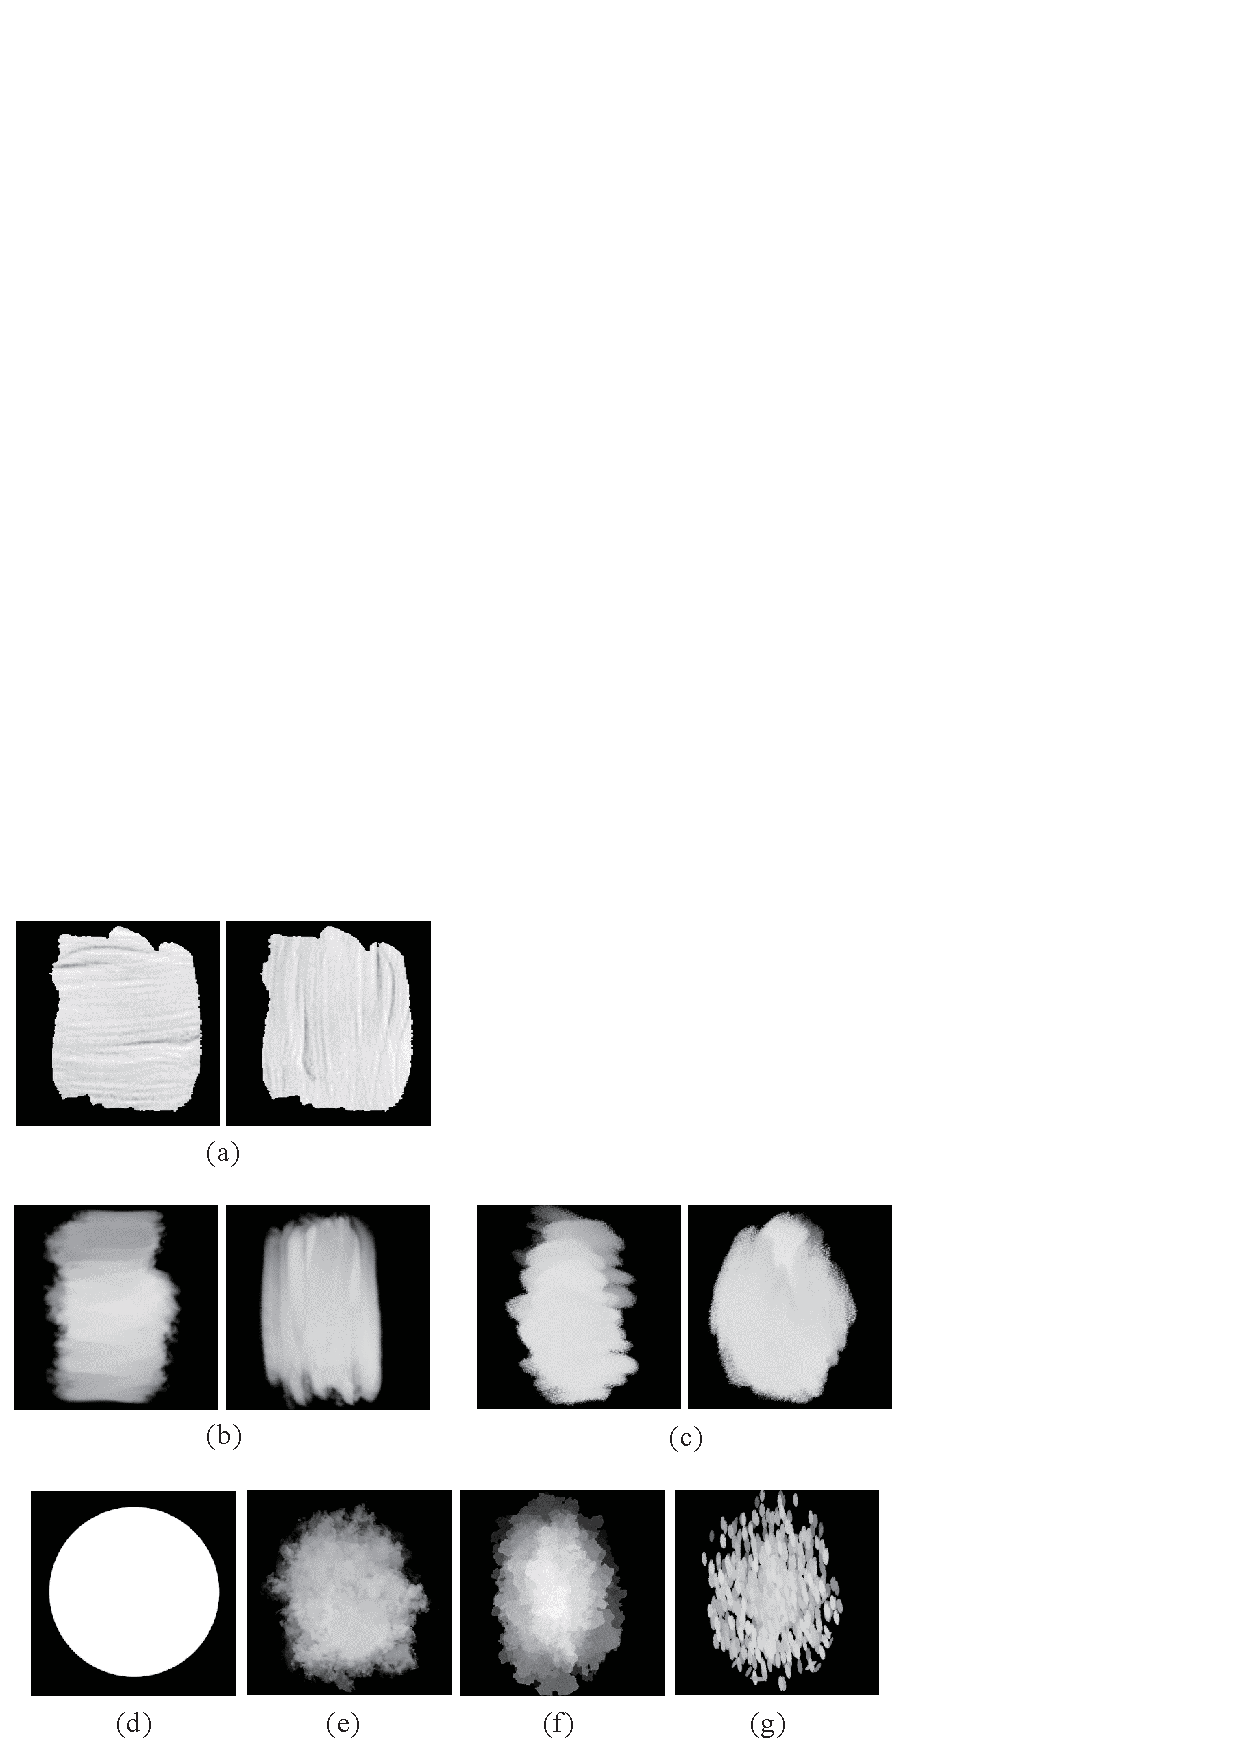
\includegraphics[width=1.0\linewidth]{resource/brushes.pdf}
    \caption{スタイル参照画像のブラシスタイルを正確に模倣するために作成した複数のブラシ画像.}
    \label{fig:brushes}
\end{figure}

\subsection{損失関数}
Paint transformerによって生成された出力画像とスタイル参照画像のブラシスタイルを評価
する損失関数として, グラム行列 (式\eqref{gram}) のL1損失
を採用した. グラム行列を用いることで, 画像の広範囲の相関を考慮することが可能
となるため, ブラシスタイルの評価に適していると判断した.

\begin{equation}
    G_{i j} = \sum_k F_{i k} F_{j k} 
    \label{gram}
\end{equation}
ここで, $F$ はブラシスタイルの評価対象の画像を示す. 

\begin{figure}[t]
    \centering
    \includegraphics[width=1.0\linewidth]{resource/inputimg.pdf}
    \caption{実験に用いたコンテンツ参照画像とスタイル参照画像.}
    \label{fig:inputs}
\end{figure}

\begin{figure}[t]
    \centering
    \includegraphics[width=1.0\linewidth]{resource/results.pdf}
    \caption{モデルに入力したスタイル参照画像(上)とモデルからの出力画像(中)と出力画像の一部拡大(下).}
    \label{fig:result}
\end{figure}

\section{実験と結果}

\subsection{実験}
提案モデルはコンテンツ参照画像とスタイル参照画像を取り込み, 結果画像を出力する.
コンテンツ画像には, The Oxford-IIIT Pet Dataset\cite{oxford}の猫の画像を1枚使用した.
使用したコンテンツ参照画像とスタイル参照画像を図\ref{fig:inputs}に示す.
図\ref{fig:inputs}の(b)はピート・モンドリアンによる『赤・青・黄のコンポジション』
(1930)であり, 図\ref{fig:inputs}の(c)はフィンセント・ファン・ゴッホによる
『星月夜』(1889)である.

\subsection{結果}
図\ref{fig:brushes}に示した7種のブラシ画像を用いて図\ref{fig:inputs}の
コンテンツ参照画像を表現するストロークを生成した際に, 図\ref{fig:inputs}の
スタイル参照画像との類似度が最も高いとされた画像は図\ref{fig:result}に示す通りに
なった. これは, 図\ref{fig:result}の上段と下段の画像のブラシスタイルが類似
していることを意味するが, ブラシスタイルが模倣されているとは言い難い結果になって
いることがわかる. これは, ベースとなるブラシ画像が7つのみであったことと,
ストロークを表現するためのパラメータが最小限であることに起因していると考えられる.

出力画像に描かれた内容については, コンテンツ参照画像のものから大きく変化していないことが
確認できる. 

\section{考察}
\subsection{今後の展望}
本研究では, コンテンツ参照画像に描かれた内容をスタイル参照画像のブラシスタイルを
用いて再描画するために, Paint transformer\cite{liu2021paint}というTransformer
ベースのフレームワークを利用した. 
提案モデルでは, Paint transformerをそのまま使用してストローク予測モデルを
学習させたため, ストロークパラメータの種類もPaint transformerと同様であり,  
5つの形状パラメータと3つの色パラメータの合計8つであった. 
今後の研究では, より多くのパラメータを追加することによって, より柔軟なブラシ
ストローク表現が可能になると考えられる. 提案モデルで生成されるストロークは, 
図\ref{fig:brushes}に示したブラシ画像を拡大・縮小・回転することによって作成
されているが, ストロークはブラシ画像を連続して複数繋げるという方法で
生成することも可能である. 
例えば, ペイントソフトのCLIP STUDIO PAINT\cite{ClipStudio}では, 図\ref{fig:discussion}の右下
に示すようなストロークを描くことができるが, 単にブラシ画像の大きさを調整するだけ
では同様のストロークを生成することはできず, 図\ref{fig:discussion}の右上のような
ストロークとなってしまう. 
ストロークパラメータの種類を増やすことによってブラシの表現力を高め, 
図\ref{fig:discussion}の右下のようなストロークを生成できるようにすることで, 
スタイル参照画像のブラシスタイルを模倣した画像を生成可能になることが期待される.


\subsection{結論}
本研究では, 順伝播型ニューラルネットワークを利用して, コンテンツ参照画像の内容を
スタイル参照画像のブラシスタイルを模倣したスタイルに変換する新しいアプローチを
提案した.
最終的な目標は, ストロークパラメータとブラシパラメータの最適化を順に繰り返すモデル
を実装することであるが, 二重の最適化の実装は行えていない.
提案モデルによって生成された画像はスタイル参照画像のブラシスタイルを模倣しているもの
にはならなかったが, 二重の最適化の実装により, 本研究で得られた結果よりも
ブラシスタイルの模倣精度が向上すると考えられる.
また, 5.1章で述べたように, ストロークパラメータの種類の少なさも改善するべき点
であると考えられるため, 二重の最適化の実装とともにパラメータ数も改善することによっても
ブラシスタイルの模倣精度が向上することが期待される. 

\begin{figure}[t]
    \centering
    
\includegraphics[width=1.0\linewidth]{resource/brush_discussion.pdf}
    \caption{提案モデルで使用したブラシの画像(左)と
    ClipStudioを用いて描いたストローク(右下)と
    ClipStudioで描いたストロークにあわせてブラシ画像を引き延ばしたもの(右上).}
    \label{fig:discussion}
\end{figure}
%\input{example_paper_text_jp.tex}

\bibliographystyle{miru2022j}
\bibliography{myref}

\begin{thebibliography}{9}% 文献数が10未満の時 {9}
\bibitem{Midjourney}
“Midjourney,” Accessed: 2023-01-09. [Online]. Available: https://midjourney.com/.

\bibitem{IST}
L. A. Gatys, A. S. Ecker, and M. Bethge, “Image style transfer using
convolutional neural networks,” in Proceedings of the IEEE Conference
on Computer Vision and Pattern Recognition (CVPR), Jun. 2016.

\bibitem{Huang_2019_ICCV}
Z. Huang, W. Heng, and S. Zhou, “Learning to paint with model-based
deep reinforcement learning,” in Proceedings of the IEEE/CVF International 
Conference on Computer Vision (ICCV), Oct. 2019.

\bibitem{liu2021paint}
S. Liu, T. Lin, D. He, F. Li, R. Deng, X. Li, E. Ding, and H. Wang,
“Paint transformer: Feed forward neural painting with stroke prediction,”
in Proceedings of the IEEE International Conference on Computer Vision, 2021.

\bibitem{oxford}
O. M. Parkhi, A. Vedaldi, A. Zisserman, and C. V. Jawahar, “The
oxford-iiit pet dataset,” [Online]. Available: https://www.robots.ox.ac.uk/~vgg/data/pets/.

\bibitem{ClipStudio}
“CLIP STUDIO PAINT,” Accessed: 2023-01-09. [Online]. Available: https://www.clipstudio.net/.


\end{thebibliography}

\end{document}
